\chapter{Background} \label{Background}

\section{JPEG}

It is not the purpose of this document to give a comprehensive description of the JPEG/JFIF format, or the algorithm. Previous work about compression of JPEG images using CUDA parallel acceleration was done by Simone Pistilli: his paper \cite{simonepap} also gives a more in-depth description of the file format and compression algorithm.

JPEG is a standard for the compression of digital images. It takes the name of its creators, the Joint Photographic Experts Group. JPEG images are commonly stored in JFIF (JPEG File Interchange Format) files.

\subsection{JPEG encoding algorithm}
The JPEG compression exploits the relatively poor sensitivity of the eye to variations of high-frequency content in images. Images are converted from spacial information to frequency information in the horizontal and vertical directions, by applying the Dual Cosine Transform on blocks of 8x8 pixels, simply called "blocks". This generates an equivalent amount of data (8x8 cells)  which represents the frequency content of the original block as shown in \autoref{fig:DCT}. Cells representing small high frequency content are then dropped (i.e. set to zero) by integer multiplication with a weighting table (\autoref{fig:quantizationTable}) which can be more or less aggressive depending on desired quality. Then the block is serialized in a zig-zag order from low to high frequency (see \autoref{fig:ZigZag}, and Huffman-encoded, finally achieving compression.\\
The first cell (0, 0) of the frequency-domain block contains the zero-frequency content, or simply the average brightness of the block. It is called "DC coefficient" of the block. This cell is compressed differently from the other 63 (which compose the AC coefficient). The DC component is stored as DPCM (Differential Pulse Code Modulation), which practically means saving only the difference from the last data point (DC component of the last block). The sequence of differences restarts periodically as defined by the Restart Interval.\\
This is enough to compress single channel (i.e. black and white) images. To represent color, each channel is represented separately. While the RGB representation can be used, it is most common to represent color images in the YCbCr format (sometimes improperly called YUV in industry). The YCbCr color space separates luminance (Y) from chrominance (Cb, Cr) components, allowing then to subsample the chrominance component (for example 2:1 reduction in both axes is labeled "4:2:0") which is perfectly acceptable to the eye, allowing further data compression without perceived loss of quality.

\subsection{JPEG File Format (JFIF)}
The container format of interest is JFIF, because it is the most widespread one (any file with \texttt{.jpg} extension is a JFIF container).\\
JFIF files are made of sections which can be distinguished by the tags that precede them. Below is a list of the most important ones:
\begin{itemize}
    \item SOF (Start Of Frame): contains general information like width, height, color space.
    \item DHT (Define Huffman Table): describes a Huffman compression tree. For YCbCr there are usually four DHTs: two for the Y channel (one for AC components, the other for DC components) and two different ones for the Cb and Cr channels (again separated for DC and AC components).
    \item DQT (Define Quantization Table): describes how the low-weight, high-frequency cells are dropped. Usually there are two, one for the Y channel and another one, usually more aggressive, for Cb and Cr.
    \item DRI (Define Restart Interval): specifies how often the DC component encoding restarts from zero.
    \item (Start of) Scan: the main section, which contains the actual data. For every block
\end{itemize}

Thankfully the format is already handled by NanoJPEG, so only a superficial understanding of the format is needed. For the purpose of porting NanoJPEG to CUDA, the most important section is the Scan section.\\
The Scan section contains the actual data. Single blocks are saved as a DC difference coefficient, then the Huffman-coded AC coefficients. If no subsampling is used, blocks from each component simply follow each other (for example \{R,G,B,R,G,B...\} or \{Y,Cb,Cr,Y,Cb,Cr...\}). If chroma subsampling is used, there are less Cb and Cr blocks than Y blocks, so the blocks from different components are grouped in integer proportions into Minimum Coded Units (MCU) or Minimum Coded Blocks (MCB). For example, the scan of a 4:2:0 YCbCr JPEG will be composed of a sequence of MCUs with the structure \{Y,Y,Y,Y,Cb,Cr\}.

\begin{figure}[ht]
\centering
    \begin{minipage}[b]{0.4\linewidth}
    \centering
    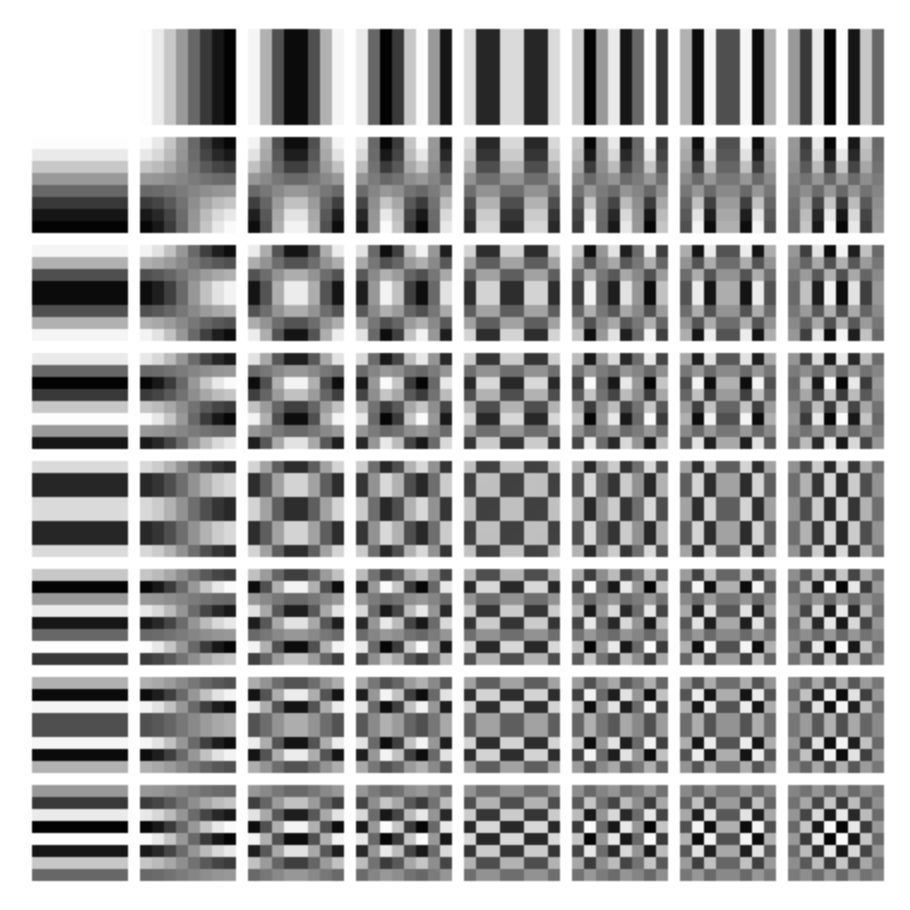
\includegraphics[width=\textwidth]{Pictures/DCT.png}
    \caption{DCT representation of an MCB. Each cell of the block here contains an image of the pattern it represents.}
    \label{fig:DCT}
    \end{minipage}
\hspace{0.05\linewidth}
    \begin{minipage}[b]{0.25\linewidth}
    \centering
    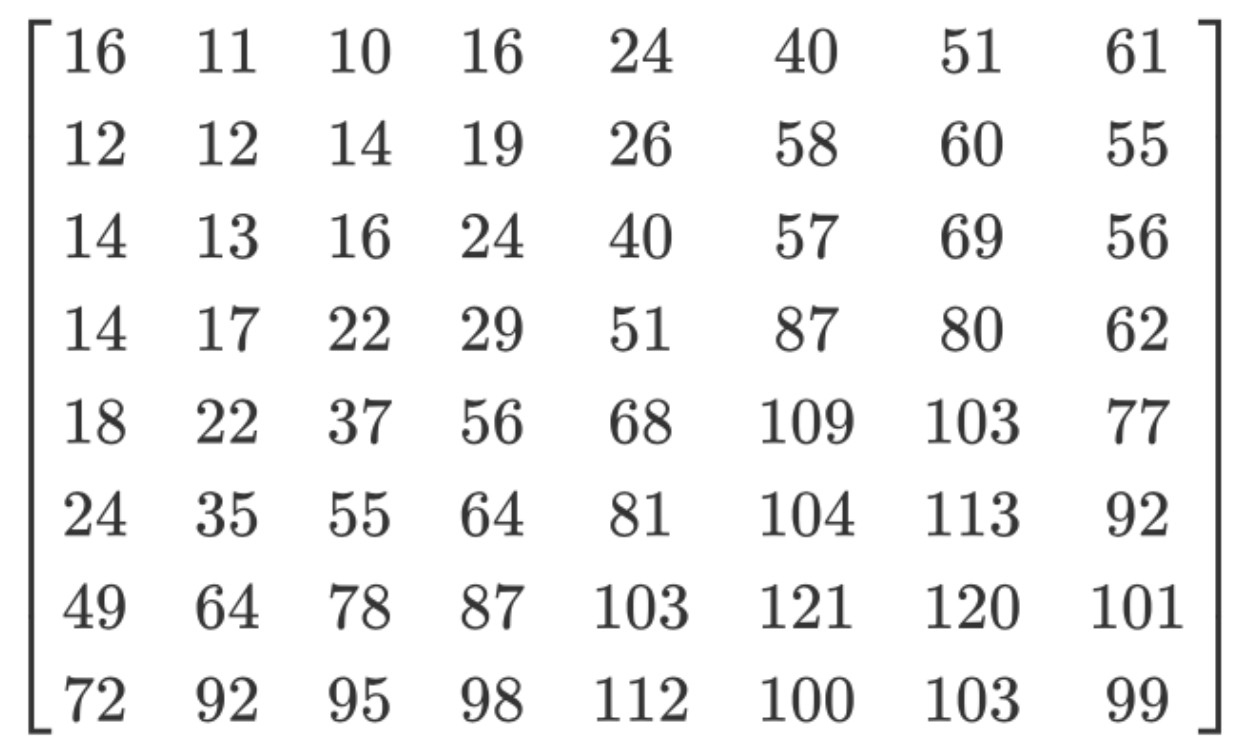
\includegraphics[width=\textwidth]{Pictures/quantization_table.png}
    \caption{Example Quantization Table. Every cell of a 8x8 frequency-domain block is divided by the value in the corresponding cell of the quantization table}
    \label{fig:quantizationTable}
    \end{minipage}
\hspace{0.05\linewidth}
    \begin{minipage}[b]{0.24\linewidth}
    \centering
    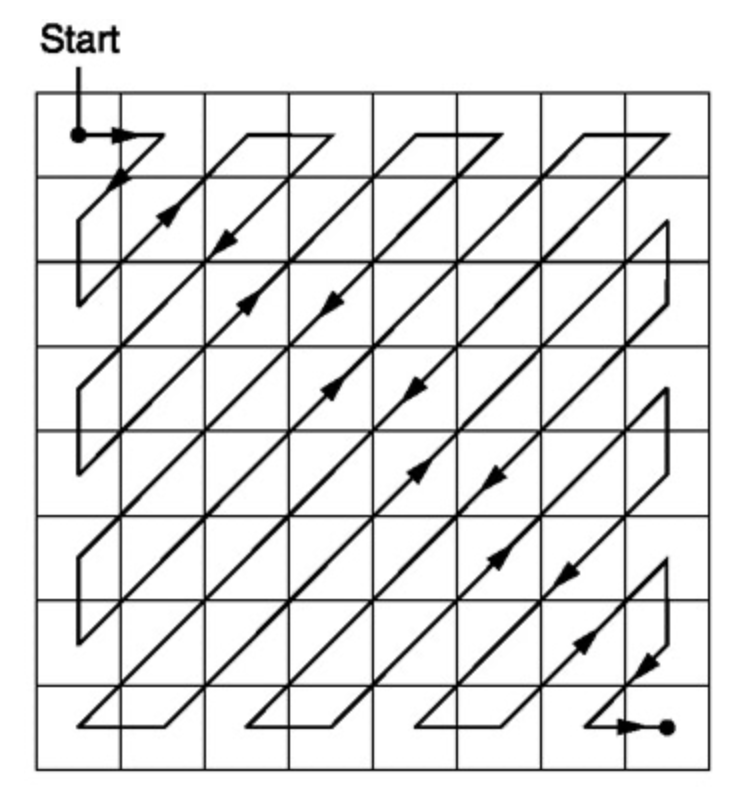
\includegraphics[width=\textwidth]{Pictures/ZigZag.png}
    \caption{Zig-Zag order for the serialization of the frequency-domain blocks}
    \label{fig:ZigZag}
    \end{minipage}
\end{figure}
